\chapter{The Evening of the Betrothal}

Villefort had, as we have said, hastened back to Madame de
Saint-Méran’s in the Place du Grand Cours, and on entering the house
found that the guests whom he had left at table were taking coffee in
the salon. Renée was, with all the rest of the company, anxiously
awaiting him, and his entrance was followed by a general exclamation.

“Well, Decapitator, Guardian of the State, Royalist, Brutus, what is
the matter?” said one. “Speak out.”

“Are we threatened with a fresh Reign of Terror?” asked another.

“Has the Corsican ogre broken loose?” cried a third.

“Marquise,” said Villefort, approaching his future mother-in-law, “I
request your pardon for thus leaving you. Will the marquis honor me by
a few moments’ private conversation?”

“Ah, it is really a serious matter, then?” asked the marquis, remarking
the cloud on Villefort’s brow.

“So serious that I must take leave of you for a few days; so,” added
he, turning to Renée, “judge for yourself if it be not important.”

“You are going to leave us?” cried Renée, unable to hide her emotion at
this unexpected announcement.

“Alas,” returned Villefort, “I must!”

“Where, then, are you going?” asked the marquise.

“That, madame, is an official secret; but if you have any commissions
for Paris, a friend of mine is going there tonight, and will with
pleasure undertake them.” The guests looked at each other.

“You wish to speak to me alone?” said the marquis.

“Yes, let us go to the library, please.” The marquis took his arm, and
they left the salon.

“Well,” asked he, as soon as they were by themselves, “tell me what it
is?”

“An affair of the greatest importance, that demands my immediate
presence in Paris. Now, excuse the indiscretion, marquis, but have you
any landed property?”

“All my fortune is in the funds; seven or eight hundred thousand
francs.”

“Then sell out—sell out, marquis, or you will lose it all.”

\begin{figure}[h]
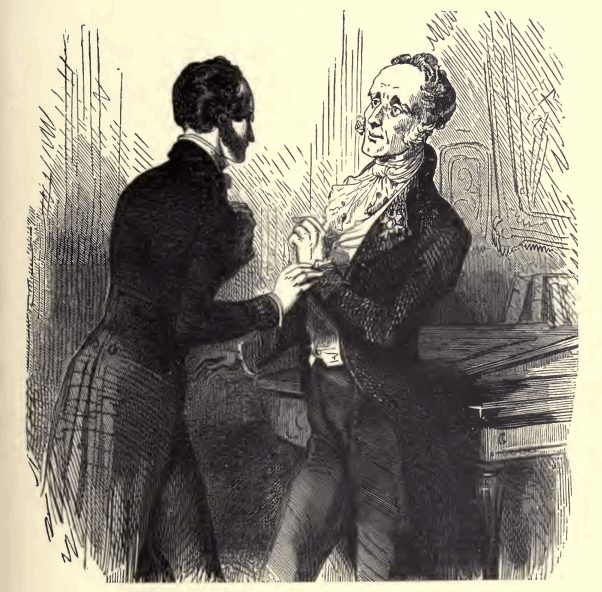
\includegraphics[width=\textwidth]{0123m.jpg}
\end{figure}

“But how can I sell out here?”

“You have a broker, have you not?”

“Yes.”

“Then give me a letter to him, and tell him to sell out without an
instant’s delay, perhaps even now I shall arrive too late.”

“The deuce you say!” replied the marquis, “let us lose no time, then!”

And, sitting down, he wrote a letter to his broker, ordering him to
sell out at the market price.

“Now, then,” said Villefort, placing the letter in his pocketbook, “I
must have another!”

“To whom?”

“To the king.”

“To the king?”

“Yes.”

“I dare not write to his majesty.”

“I do not ask you to write to his majesty, but ask M. de Salvieux to do
so. I want a letter that will enable me to reach the king’s presence
without all the formalities of demanding an audience; that would
occasion a loss of precious time.”

“But address yourself to the keeper of the seals; he has the right of
entry at the Tuileries, and can procure you audience at any hour of the
day or night.”

“Doubtless; but there is no occasion to divide the honors of my
discovery with him. The keeper would leave me in the background, and
take all the glory to himself. I tell you, marquis, my fortune is made
if I only reach the Tuileries the first, for the king will not forget
the service I do him.”

“In that case go and get ready. I will call Salvieux and make him write
the letter.”

“Be as quick as possible, I must be on the road in a quarter of an
hour.”

“Tell your coachman to stop at the door.”

“You will present my excuses to the marquise and Mademoiselle Renée,
whom I leave on such a day with great regret.”

“You will find them both here, and can make your farewells in person.”

“A thousand thanks—and now for the letter.”

The marquis rang, a servant entered.

“Say to the Comte de Salvieux that I would like to see him.”

“Now, then, go,” said the marquis.

“I shall be gone only a few moments.”

Villefort hastily quitted the apartment, but reflecting that the sight
of the deputy procureur running through the streets would be enough to
throw the whole city into confusion, he resumed his ordinary pace. At
his door he perceived a figure in the shadow that seemed to wait for
him. It was Mercédès, who, hearing no news of her lover, had come
unobserved to inquire after him.

As Villefort drew near, she advanced and stood before him. Dantès had
spoken of Mercédès, and Villefort instantly recognized her. Her beauty
and high bearing surprised him, and when she inquired what had become
of her lover, it seemed to him that she was the judge, and he the
accused.

“The young man you speak of,” said Villefort abruptly, “is a great
criminal, and I can do nothing for him, mademoiselle.” Mercédès burst
into tears, and, as Villefort strove to pass her, again addressed him.

“But, at least, tell me where he is, that I may know whether he is
alive or dead,” said she.

\begin{figure}[h]
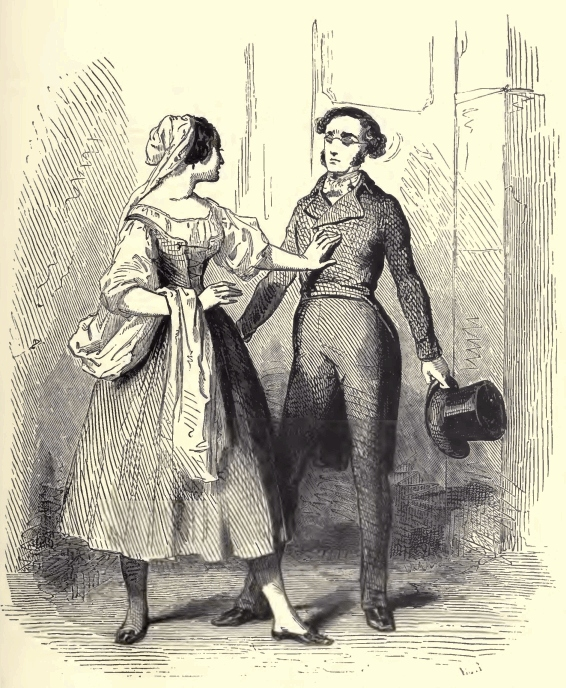
\includegraphics[width=\textwidth]{0125m.jpg}
\end{figure}

“I do not know; he is no longer in my hands,” replied Villefort.

And desirous of putting an end to the interview, he pushed by her, and
closed the door, as if to exclude the pain he felt. But remorse is not
thus banished; like Virgil’s wounded hero, he carried the arrow in his
wound, and, arrived at the salon, Villefort uttered a sigh that was
almost a sob, and sank into a chair.

Then the first pangs of an unending torture seized upon his heart. The
man he sacrificed to his ambition, that innocent victim immolated on
the altar of his father’s faults, appeared to him pale and threatening,
leading his affianced bride by the hand, and bringing with him remorse,
not such as the ancients figured, furious and terrible, but that slow
and consuming agony whose pangs are intensified from hour to hour up to
the very moment of death. Then he had a moment’s hesitation. He had
frequently called for capital punishment on criminals, and owing to his
irresistible eloquence they had been condemned, and yet the slightest
shadow of remorse had never clouded Villefort’s brow, because they were
guilty; at least, he believed so; but here was an innocent man whose
happiness he had destroyed. In this case he was not the judge, but the
executioner.

As he thus reflected, he felt the sensation we have described, and
which had hitherto been unknown to him, arise in his bosom, and fill
him with vague apprehensions. It is thus that a wounded man trembles
instinctively at the approach of the finger to his wound until it be
healed, but Villefort’s was one of those that never close, or if they
do, only close to reopen more agonizing than ever. If at this moment
the sweet voice of Renée had sounded in his ears pleading for mercy, or
the fair Mercédès had entered and said, “In the name of God, I conjure
you to restore me my affianced husband,” his cold and trembling hands
would have signed his release; but no voice broke the stillness of the
chamber, and the door was opened only by Villefort’s valet, who came to
tell him that the travelling carriage was in readiness.

Villefort rose, or rather sprang, from his chair, hastily opened one of
the drawers of his desk, emptied all the gold it contained into his
pocket, stood motionless an instant, his hand pressed to his head,
muttered a few inarticulate sounds, and then, perceiving that his
servant had placed his cloak on his shoulders, he sprang into the
carriage, ordering the postilions to drive to M. de Saint-Méran’s. The
hapless Dantès was doomed.

As the marquis had promised, Villefort found the marquise and Renée in
waiting. He started when he saw Renée, for he fancied she was again
about to plead for Dantès. Alas, her emotions were wholly personal: she
was thinking only of Villefort’s departure.

She loved Villefort, and he left her at the moment he was about to
become her husband. Villefort knew not when he should return, and
Renée, far from pleading for Dantès, hated the man whose crime
separated her from her lover.

\begin{figure}[h]
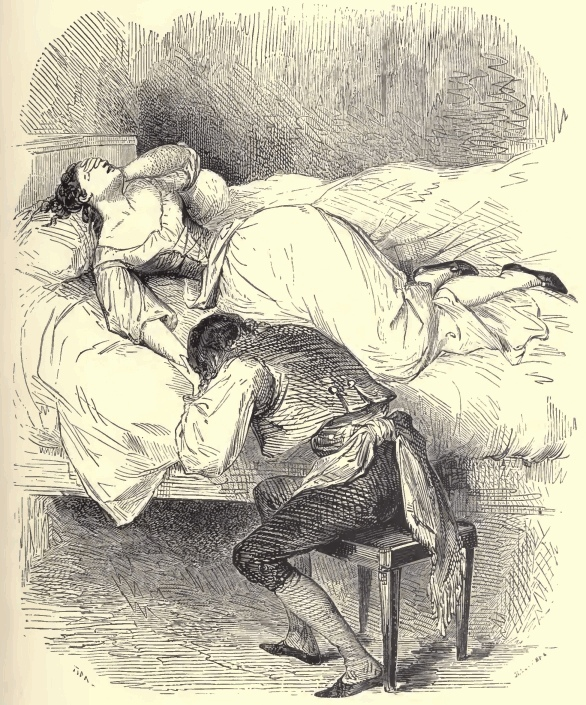
\includegraphics[width=\textwidth]{0127m.jpg}
\end{figure}

Meanwhile what of Mercédès? She had met Fernand at the corner of the
Rue de la Loge; she had returned to the Catalans, and had despairingly
cast herself on her couch. Fernand, kneeling by her side, took her
hand, and covered it with kisses that Mercédès did not even feel. She
passed the night thus. The lamp went out for want of oil, but she paid
no heed to the darkness, and dawn came, but she knew not that it was
day. Grief had made her blind to all but one object—that was Edmond.

“Ah, you are there,” said she, at length, turning towards Fernand.

“I have not quitted you since yesterday,” returned Fernand sorrowfully.

M. Morrel had not readily given up the fight. He had learned that
Dantès had been taken to prison, and he had gone to all his friends,
and the influential persons of the city; but the report was already in
circulation that Dantès was arrested as a Bonapartist agent; and as the
most sanguine looked upon any attempt of Napoleon to remount the throne
as impossible, he met with nothing but refusal, and had returned home
in despair, declaring that the matter was serious and that nothing more
could be done.

Caderousse was equally restless and uneasy, but instead of seeking,
like M. Morrel, to aid Dantès, he had shut himself up with two bottles
of black currant brandy, in the hope of drowning reflection. But he did
not succeed, and became too intoxicated to fetch any more drink, and
yet not so intoxicated as to forget what had happened. With his elbows
on the table he sat between the two empty bottles, while spectres
danced in the light of the unsnuffed candle—spectres such as Hoffmann
strews over his punch-drenched pages, like black, fantastic dust.

Danglars alone was content and joyous—he had got rid of an enemy and
made his own situation on the \textit{Pharaon} secure. Danglars was one of
those men born with a pen behind the ear, and an inkstand in place of a
heart. Everything with him was multiplication or subtraction. The life
of a man was to him of far less value than a numeral, especially when,
by taking it away, he could increase the sum total of his own desires.
He went to bed at his usual hour, and slept in peace.

Villefort, after having received M. de Salvieux’s letter, embraced
Renée, kissed the marquise’s hand, and shaken that of the marquis,
started for Paris along the Aix road.

Old Dantès was dying with anxiety to know what had become of Edmond.
But we know very well what had become of Edmond.
